
\section{Background}

In their paper Vinyals et al\cite{DBLP:journals/corr/VinyalsL15} discuss making a chatbot using a neural network configured for sequence to sequence neural machine translation. An attempt to code our own sequence to sequence model was not very fruitful so instead we use code authored by Inkawhich et al\cite{2018Inkawhich}.

In their paper Vaswani et al\cite{Vaswani2017AttentionIA} discuss using the Transformer architecture for solving machine learning tasks. We train a transformer model as a chatbot. We adopt this model to create a chatbot.

Also Radford et al\cite{radford2019language} discuss the `Generative Pre-training Transformer 2' (GPT2) neural network for Natural Language Processing (\ac{NLP}) tasks. The GPT2 model is based largely on the Transformer architecture. 

We implement a chatbot with a GPT2 model. We use a program library from Wolf et al\cite{Wolf2019HuggingFacesTS} to run our model.

It is worth noting that with the appearance of the Transformer architecture and WordPiece vocabulary scheme, some traditional technologies have become redundant or obsolete. This may be true of any model that uses Recurrent Neural Network components and also the traditional word vector embeddings.

\section{Recurrent Neural Network Components}

\subsection*{Overview}
The goal behind Recurrent Neural Network (RNN) components is to detect patterns. Since understanding RNNs is important to GPT2 and Transformer models, we discuss RNNs here. Here we explore a simple \ac{RNN} first. 

The simplest Recurrent Neural Network has two inputs and two outputs. They can be arranged in patterns. In our example the input will be a sequence of data and the Recurrent Neural Network will be a line of components of the same length as the data.

One input from each component is the hidden state output from the Recurrent Neural Network to the left. Another input is the current input from the sequence that the component is encoding. One output is the generated hidden state, meant for the component to the right. The last output is the value that the Recurrent Neural Network outputs or surmises. 

\begin{figure}[H]
	\begin{center}
	
	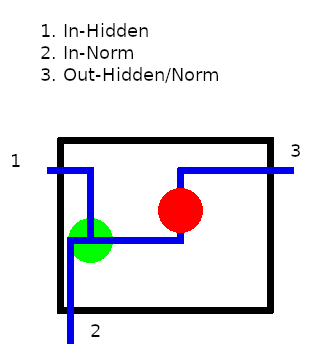
\includegraphics[scale=0.5]{diagram-rnn}
		
	\end{center}
	\caption[Recurrent Neural Network]{RNN - 1 and 2 are inputs, 3 is the output.}
	

\end{figure}

In our diagram the two inputs are labeled 1 and 2, and the single output does double duty as both the hidden state output and the value that the Recurrent Neural Network outputs or surmises.

There are several designs for a Recurrent Neural Network component. The inner workings of these components are what makes them different. In the example in the diagram the inner workings are very simple. Two paths, labeled as inputs, take data into the Recurrent Neural Network. Their data is combined in the green circle. This combination is done with concatenation and simple feed forward neural network components. The output from the concatenation is passed through the red circle. This is a `tanh' activation operation that limits the output to values from -1 through 1. This `tanh' activation keeps the output within reasonable values. Finally the output is delivered outside the component to the program employing the Recurrent Neural Network. In this diagram there is only one output. The single output would serve as both the hidden state output for that position in the encoder or decoder, and also the data output component for that position.



\subsection*{Gated Recurrent Unit}
An implementation of a Recurrent Neural Network is the `Gated Recurrent Unit' (GRU). There are other varieties of RNN, most notably the Long Short Term Memory (LSTM) cell. We do not explore \ac{LSTM} cells here.

A \ac{GRU} has two inputs and two outputs. The formulas for a Gated Recurrent Unit, as outlined by Denny Britz in the website WILDML (Britz et al)\cite{2015Britz}, are as follows.

\begin{minipage}{5in}

$$ z =\sigma(x_tU^z + s_{t-1} W^z) $$  
$$ r =\sigma(x_t U^r +s_{t-1} W^r) $$  
$$ h = tanh(x_t U^h + (s_{t-1} \circ r) W^h) $$  
$$ s_t = (1 - z) \circ h + z \circ s_{t-1} $$  

\end{minipage}

\bigskip \bigskip

The Gated Recurrent Unit has two inputs and two outputs. It also has two internal gates. One internal gate is the `reset' gate. This one determines how much of the previous input is combined with the new value calculated by the mechanism of the Gated Recurrent Unit. It is denoted as `$r$' above. Another internal gate is the `update' gate. The update gate decides how much new information is to be included in gate computation. It is denoted as `$z$'.

Here `$ s_t $' is the symbol for the output. The two inputs are `$ x_t $' and `$ s_{t-1} $' . `$ x_t $' is the hidden state input. `$ s_{t-1} $' is the regular input for the Recurrent Neural Network or Gated Recurrent Unit. Sigmoid activation is used on the two gates, using the symbol `$ \sigma(...) $' , while tanh activation is used to compute the hidden output. The hidden output is found in the third line, denoted as `$h$'.

The dimension of the $U^z$, $U^r$ and $U^h$ matrices is the hidden unit size by the hidden unit size. $ x_t $ is a vector the size of the hidden unit. The $U$ values, along with $ W^z $, $ W^r $ and $ W^h $  are all simple matrices that allow the GRU to operate.

In the last line, the regular output is determined using the `dot' product which is denoted with a circle, along with an addition operation. In the two gate formulas (the first and second) the output is determined as the sum of two matrix multiplication operations passed through sigmoid activation. This produces values in the range of 0 to 1.

Under most programming circumstances the Gated Recurrent Unit is not implemented by the average programmer. The programmer employs a language like python and a programming library like Pytorch or Tensorflow. The library then implements the Gated Recurrent Unit and makes it easy for the programmer to use that implementation.

\section{Sequence to Sequence}

Translating text from one language to another has become a common task for computers. The Sequence to Sequence architecture is often used today for this purpose. Here we explain how this works.

A naive approach to translation involves using a dictionary. You would encode each key as a word from one language and the value for that key would be the translated word in the target language. Of course this doesn't work, because different languages not only have different words for the same thing, but they also have different sentence structures for what might be similar concepts.

A better approach is sequence to sequence translation. A description follows with a section at the end for how training works.

In this approach we use recurrent neural networks to obtain our translation. Two recurrent neural network components are employed. One is responsible for the input language and the other for the output. 

\iffalse
\subsection*{Formula}
Below is a product formula. It says that the $y_n$ term relies on the sequence of terms that starts with $y_1$ and continues to $y_{n-1}$. It also has $v$ that represents the 'thought vector' which is present along with $y_1,...,y_{t-1}$ as an input to the decoder Gated Recurrent Unit and helps formulate $y_t$.

On the left side of the formula we have $x_1,...x_T$ which represents the input sequence for the encoder. Also we have $y_1,...,y_{T'}$ which represents the entire output. $T$ is the length of the input while $T'$ is the length of the output. Those two $T$ terms do not need to be the same, and often are not. Again, $v$ is the hidden state passed from the encoder to the decoder as a 'thought vector'.

\[
\mathlarger{ \mathlarger{ \mathlarger{
			p(y_1,...,y_{T'}|x_1,...,x_T) = \prod_{t=1}^{T'} p(y_t|v,y_1,..., y_{t-1}) 
} } }
\]

Every prediction relies on all the previous predictions up until that point. This is what happens in sequence to sequence and transformer architectures when the model is producing output. 

The probability for the entire output is the same as the product of the probability of each word as it is generated. 

%We include this formula in place of a flow chart.

This function can be found in Sutskever et al\cite{DBLP:journals/corr/SutskeverVL14}.

\fi

\subsection*{Word Embeddings}

Also employed are two vocabulary sets. One vocabulary is for the source language and another is for the target language. A table of word vectors the size of the input vocabulary is created and a maximum sentence length is picked. There is also a `hidden size', which is an important dimension in the model. In practice the hidden size could be 300 units and more for this kind of application.

Words are translated from strings to individual numbers from a vocabulary dictionary. The dictionary only contains a single unique number for every word. Then the number is passed through an embedding structure. This turns the single number into a vector of numbers that is the same size as the RNN hidden dimension. Then, from that time on the model uses the vector instead of words.

The contents of the embedding unit is a table of numbers, all are of the size of the RNN hidden dimension. The vectors are usually, but don\textquoteright t have to be, unique values. There is one complete hidden dimension sized vector for each word in the vocabulary. 

\begin{figure}[H]
	\begin{center}
		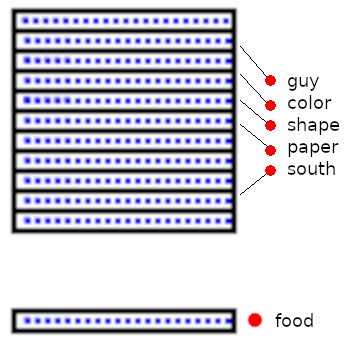
\includegraphics[scale=0.5]{diagram-embedding}
		
		
	\end{center}
	\caption[Word Embeddings]{Embeddings - Each word from a dictionary is converted to a vector of numbers.}
	

\end{figure}

The vectors can be initialized randomly or they can be filled with predetermined values. As the network trains the embedding values can either be modified or frozen in place. Typically if the contents were initialized randomly the values would be trained. If the contents were filled with predetermined values you don\textquoteright t want to train them or change them in any way. 

There are at this writing two main types of pretrained word embeddings. One is called \textquoteleft Word2Vec\textquoteright{} and one is called \textquoteleft GloVe\textquoteright . 

Word2Vec is short for \textquoteleft Word to Vector.\textquoteright{} (Mikolov et al.)\cite{mikolov2013efficient} GloVe is short for \textquoteleft Global Vector.\textquoteright{} (Pennington et al.)\cite{pennington-etal-2014-glove} .

Word vectors are created composed of floating point numbers. Each word in the vocabulary is translated to an integer which remains the same throughout the use of the translator. The word vectors are arranged in a table of floating point numbers with one dimension being the size of the input vocabulary and one dimension being the hidden size for the vector.

\subsection*{Corpus}

A text must be prepared for training. A text corpus with source and target pairs is chosen. Sentences in the source corpus are paired with sentences with the same meaning in the target corpus. Sentence length is observed and for all sentences shorter than that length a special `end-of-sequence' token is appended to all sequences. This restriction is applied in both languages.

\subsection*{Input Tokens}

So far the model takes a word, translates it to an integer, and finds the vector in the word embedding table that represents that word. It does this for the first word and all subsequent words one by one. Then it gives the entire vector for a word to the GRU, one at a time. The GRU takes the word and passes it to some inner components. It decides weather to return as output just the input or the input modified. This is what the Gated Recurrent Unit does internally.

The Gated Recurrent Unit takes as input two vectors. It processes the `input' vector and returns another vector. This could be exactly the same as the input but is usually somehow changed. The input vector and the output vector have the dimension of the `hidden size' mentioned above. Throughout the discussion of this model the hidden size will remain the same. The Gated Recurrent Unit also operates on two hidden states. One hidden state, a vector, is taken in and another hidden state, also a vector, is produced for output.

We will describe components in two groups. The input components, from the source language, are the encoder and the output components, from the target language, are the decoder.



\subsection*{Encoder}

The input segments, composed of Gated Recurrent Units, take two input vectors and return two output vectors. One input is the vector from the embedding table. Another input vector is the previous hidden state. The hidden state is the same size as the input from the embedding table, but typically it comes from the previous Gated Recurrent Unit. The output vector is a hidden value for the Recurrent Unit to the right.

The very first Gated Recurrent Unit in the input chain ignores the fact that the first word has no hidden value. It consumes the first word vector. Then it passes it's output to the next Gated Recurrent Unit in the chain. This Gated Recurrent Unit uses the output of the previous Gated Recurrent Unit as the hidden value. It also uses the vector for the second word. It passes it's important information to the Gated Recurrent Unit to it's right. Then the last Gated Recurrent Unit in the encoder passes it's hidden state to the output chain, the decoder.

A complicating detail is that although many Gated Recurrent Units are called for in the encoder they all use the same set of weights and biases. For this reason only a single input Gated Recurrent Unit is used for all of the words in practice. Outputs are calculated and then cycled around and fed with the next word from the sentence in vector form to the input of the Gated Recurrent Unit. 

\subsection*{Decoder}
The output is in charge of generating tokens that represent, in this case, the translation of the input to the output language. The output uses Gated Recurrent Unit segments also. The first hidden input for the first output cell is taken from the last hidden output of the last recursive unit of the input. It is important because it is the spot where a great amount of data is passed from the encoder to the decoder. The connection at this point is said to carry the `thought vector'. Most of the information responsible for translating one language to another is passed at this point.

The hidden values from the input section are passed to the first output Gated Recurrent Unit. It outputs the values that are later converted to the first word of the output. The first output Gated Recurrent Unit also has a hidden state. It passes the first word and the hidden state on to the second Gated Recurrent Unit.

The second Gated Recurrent Unit generates the second word and also its own hidden state. The second word is recorded and the word and the hidden state are passed on to the next Gated Recurrent Unit. This is repeated until a special `end-of-sequence' token is found or until the number of tokens equals the maximum number allowed.

\begin{figure}[H]
	\begin{center}
	
	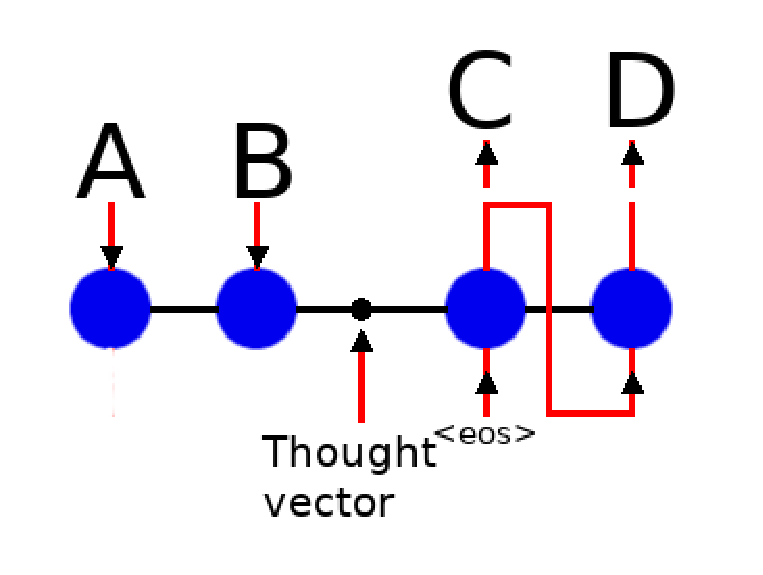
\includegraphics[scale=0.5]{diagram-nmt}
		
\end{center}
	\caption[Sequence to Sequence Architecture]{Seq2seq: A and B represent an input sequence and C and D represent the corresponding output.}
	

\end{figure}

In this figure we generalize a sequence to sequence model. The idea is that A and B, on the left side of the diagram, deal with the encoding of sentences. A and B would be consecutive words in a sentence, and the round blue nodes below A and B are Recurrent Neural Network units. C and D are outputs and in the right side of the diagram the blue nodes represent the output Recurrent Neural Network units. Between the input and the output there is a corridor of information exactly the size of the Recurrent Neural Network hidden vector. 

All of the information that the decoder uses for it\textquoteright s output is present in this corridor and is passed along the corridor from the encoder. For this reason we refer to it as the thought vector. We will see later that aside from Attention Mechanisms, there is no other place where information is passed from the encoder to the decoder.

Making this vector larger by increasing the size of the hidden dimension allows for more information in the thought vector. Size also increases the time to train the network. The size must also match the dimension of the vectors in the GloVe or Word2Vec download if one of those is used. 

Ultimately exceedingly large hidden dimension does not improve the sequence to sequence model.

Again in the Decoder, many GRU units are called for but they all share the same weights and biases. For this reason a single GRU is employed for the entire Decoder.

\subsection*{Output Tokens}
Each output we have is currently in the form of a vector. These vectors are a long string of floating point numbers, each one the dimensions of the `hidden size' mentioned above. What's done with them is they are converted to the dimensions of the output vocabulary, through matrix multiplication. Then they are processed in what is called an `arg-max' function. This processing determines the index of the maximum value in the new vocabulary sized vector. This index allows the program to look up the corresponding word in the output vocabulary. This word is then used as the model output at that point in the output chain.

There are some inherent problems. Because the output of a Gated Recurrent Unit is constantly being reused as the input, lots of data that might be useful to have is lost when the Gated Recurrent Unit churns through internal operations where several matrix multiplication operations are performed together on input. With every iteration more data is lost and so, for example, the effective length of the input and output sentences must be short. 

Another problem is that all input to be translated to target output has to be boiled down and passed to the output section through a small corridor the size of a typical word vector. This channel is sometimes referred to as the `thought vector.' Without attention, described below, all necessary information must be right there. This also limits the length of the input and output vectors. It does help, when setting up a model for later training, to make the hidden size larger, but it only helps so much. There is a point at which the benefit of increasing the hidden size is lost.

This is how some computer models do language translation. Using `arg-max' is an example of a greedy approach. Another approach might use something like `Beam Selection' but we're not going to get into that here.


\section{Loss and Accuracy During Training}

At first the prediction from a model is not very close to the desired output. The output is compared to the prediction and a `loss' is generated. `Loss' measures the difference between the predicted output and the target. A larger loss represents two values, prediction and target, that are further apart. 

Another metric is Accuracy. `Accuracy' is a numerical representation of the difference between the desired output and the generated prediction. It is a percentage of the time that the output is exactly correct.

Getting a prediction, running input data through a neural network, is forward propagation. Training, then, is a mathematical process involving backpropagagtion. Backpropagation identifies areas of the model weights that need to be modified in order to get the proper prediction in the future.

We take the derivative of the loss function in order to backpropagate. The derivative is manipulated with the learning rate. The original weight value is changed minutely. The amount changed with every backward propagation is dependent on the learning rate. The result is a set of adjusted weight matrices and a new loss. When these matrices are used later they allow for better predictions. 

This is done over and over with every source/target sentence pair. Slowly the model is changed and predictions start to match the target. That's training. The loss should decrease over time and the accuracy should increase.

There are several numerical metrics that we can record during training that tell us how our model is training. The loss, a mathematical calculation of the difference between the model's output and the predicted value, is mentioned above. Loss is an important number. Also accuracy is important. Accuracy is a mathematical calculation of the difference between the model's output and the value that output should be, but it focuses on the number of times the model comes out with a correct prediction verses how many output values there are in total.

\section{Attention Mechanism}

Attention Mechanisms are used by sequence to sequence models to transfer more information from the encoder to the decoder. As stated above there is only one place where the encoder imparts information on the decoder, the `thought vector'. Attention helps the encoder tell the decoder which word is more important. This stressing of a vector by the model is the attention mechanism attending to one output.

Here we consider a simple attention mechanism that is used in the Sequence to Sequence model by Inkawhich et al.\cite{2018Inkawhich}. The concept for this attention comes from Luong et al\cite{DBLP:journals/corr/LuongPM15}.

Luong et al\cite{DBLP:journals/corr/LuongPM15} are interested in three kinds of calculation for their attention mechanism. The three methods use slowly increasing levels of complication. First they propose a method that just uses the dot product. Then they propose a method that just uses a field of weights. Finally they use a method that uses concatenation, along with a field of weights and a pass through a `tanh' activation layer.

$$
\boldmath
score(h_t^ \text{,} \bar{h}_s) =
\begin{cases}
    h_t^\intercal \bar{h}_s & \text{dot} \\
	h_t^\intercal W_a \bar{h}_s & \text{general} \\
	v_a^\intercal \text{tanh}(W_a [h_t ; \bar{h}_s] ) & \text{concat}
\end{cases}
\unboldmath
$$

Here $h_t$ is the symbol for the output of the current decoder and $\bar{h}_s $ is the symbol for another output taken from the input encoder. This one is the entire set of encoder states. $h_t^\intercal$ stands for $h_t$ transposed. Inkawhich et al\cite{2018Inkawhich} uses the `dot' variety.

The formula is used after the decoder Gated Recurrent Unit calculates it's hidden state. It is below.

$$ 
\boldmath
\mathlarger{ \mathlarger{
score = h_t^\intercal \bar{h}_s 
} }
\unboldmath
$$ 

Basically the output of the current decoder is transposed. Then it is multiplied by the hidden value from the entire set of encoder states. Not pictured here, the score is multiplied by the Gated Recurrent Unit decoder output, and then passed through a `tanh' activation layer. It becomes the decoder output.

\section{Sequence to Sequence Chatbot}

Vinyals et al\cite{DBLP:journals/corr/VinyalsL15} make an interesting proposition. They say that it's possible to make what they call a Neural Conversational Model by constructing a Sequence to Sequence model, but instead of using two corpus from different languages a single language is used for both source and target.

Chatbots have for a long time been constructed using \ac{AIML}. AIML, (Artificial Intelligence Markup Language) requires hand coding individual rules for every input and response. A Neural Conversational Model would not use those sorts of rules.

To create a model like this more is required than just a single input and output language. There must be a relationship between the source and the target. We want there to be a question-and-answer-like relation. Finding a corpus like this can be difficult.

It would be easy to duplicate the input source material in the target corpus. This would produce auto-encoding. The model would learn to repeat everything that was given to it in it's output. Though the model learns a task, it is not the dynamic task we want. Conversations, on the other hand, supply the relationship we are looking for. Starting with almost any question sentence in a conversation, the sentence following it answers the question posed. 

What would be a good candidate for this kind of verbal play? Vinyals et al\cite{DBLP:journals/corr/VinyalsL15} use a movie transcript data set. Essentially they take movie dialogue and break it into sentences. Even numbered sentence are the source material, and odd numbered sentences are the target. Using this method there are times when the source and target are not from the same conversation, like times in a movie dialog when the scene switches from one locale to another. Comparing this, though, to the number of times that the two sentences are from the same dialogue, the movie transcript database serves very well.

Training for this model is relatively straight forward. There is a problem though. We can follow the loss and make sure it is decreasing, but the accuracy tells us nothing and in this case does not increase as we would like it to. The loss goes down but the accuracy does not go up.

\begin{figure}[H]
	\begin{center}
	
	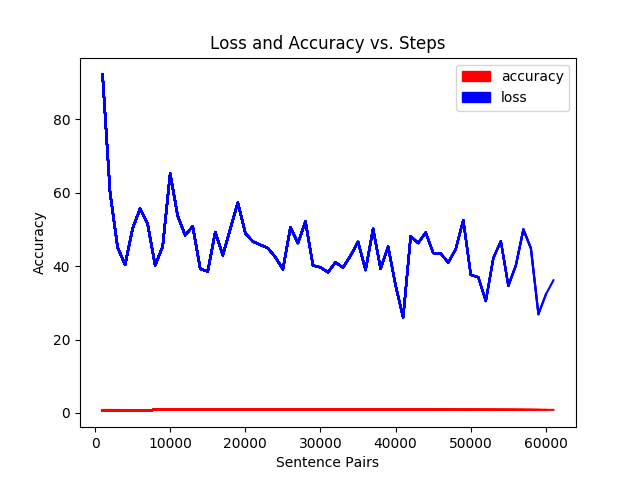
\includegraphics[scale=0.5]{Figure_1}
		
\end{center}
	\caption[Loss and Accuracy]{Loss and Accuracy: Red is accuracy and blue is loss.}
	

\end{figure}

This is because the source and target do not have the same meaning. The model does learn the task at hand but during training we have to ignore the accuracy. Success is usually measured by the accuracy of the holdout test set. Here we must measure the success with a subjective examination of the trained model.

We have to interactively give the model questions that we might ask someone that we are having a conversation with, and then see how it answers. Over and over we have to test the model. If we are satisfied with the answers then the training was a success.